\documentclass[11pt]{article}
\usepackage{lmodern}
\usepackage{amssymb,amsmath}
\usepackage{ifxetex,ifluatex}
%\usepackage{fixltx2e} % provides \textsubscript
\usepackage{xr} % referencing external ducument
\ifnum 0\ifxetex 1\fi\ifluatex 1\fi=0 % if pdftex
  \usepackage[T1]{fontenc}
  \usepackage[utf8]{inputenc}
\else % if luatex or xelatex
  \ifxetex
    \usepackage{mathspec}
  \else
    \usepackage{fontspec}
  \fi
  \defaultfontfeatures{Ligatures=TeX,Scale=MatchLowercase}
\fi
% use upquote if available, for straight quotes in verbatim environments
\IfFileExists{upquote.sty}{\usepackage{upquote}}{}
% use microtype if available
\IfFileExists{microtype.sty}{%
\usepackage{microtype}
\UseMicrotypeSet[protrusion]{basicmath} % disable protrusion for tt fontshttps://de.overleaf.com/project/5e85b0680d0bed00011ea790
}{}
\usepackage[margin=1in]{geometry}
\usepackage{hyperref}
\hypersetup{unicode=true,
            pdftitle={Title: Limitations to the Human Neandertal Admixture dating Supplements},
            pdfauthor={Leonardo Nicola Martin Iasi (Max Planck Institute for Evolutionary Anthropology, MPI EVA), Dr.~Benjamin Marco Peter (MPI EVA, benjamin\_peter@eva.mpg.de)},
            pdfborder={0 0 0},
            breaklinks=true}
\urlstyle{same}  % don't use monospace font for urls
 
\usepackage{natbib}
\bibliographystyle{References/my_abbrvnat}
\setcitestyle{authoryear,open={(},close={)}}

\usepackage{graphicx,grffile}
\makeatletter
\def\maxwidth{\ifdim\Gin@nat@width>\linewidth\linewidth\else\Gin@nat@width\fi}
\def\maxheight{\ifdim\Gin@nat@height>\textheight\textheight\else\Gin@nat@height\fi}
\makeatother
% Scale images if necessary, so that they will not overflow the page
% margins by default, and it is still possible to overwrite the defaults
% using explicit options in \includegraphics[width, height, ...]{}

\setkeys{Gin}{width=\maxwidth,height=\maxheight,keepaspectratio}
\IfFileExists{parskip.sty}{%
\usepackage{parskip}
}{% else
\setlength{\parindent}{0pt}
\setlength{\parskip}{6pt plus 2pt minus 1pt}
}
\setlength{\emergencystretch}{3em}  % prevent overfull lines
\providecommand{\tightlist}{%
  \setlength{\itemsep}{0pt}\setlength{\parskip}{0pt}}
\setcounter{secnumdepth}{0}
% Redefines (sub)paragraphs to behave more like sections
\ifx\paragraph\undefined\else
\let\oldparagraph\paragraph
\renewcommand{\paragraph}[1]{\oldparagraph{#1}\mbox{}}
\fi
\ifx\subparagraph\undefined\else
\let\oldsubparagraph\subparagraph
\renewcommand{\subparagraph}[1]{\oldsubparagraph{#1}\mbox{}}
\fi



\usepackage{setspace}
\onehalfspacing
\usepackage[left]{lineno}
\linenumbers
\usepackage[none]{hyphenat}
\usepackage{amsfonts}
\usepackage{amssymb}
\usepackage{graphicx}
\usepackage{float}
\usepackage{xcolor}
\usepackage{booktabs}
\usepackage{longtable}
\usepackage{array}
\usepackage{multirow}
\usepackage{wrapfig}
\usepackage{float}
\usepackage{colortbl}
\usepackage{pdflscape}
\usepackage{tabu}
\usepackage{threeparttable}
\usepackage{threeparttablex}
\usepackage[normalem]{ulem}
\usepackage{makecell}

\floatplacement{figure}{H}
\begin{document}

\begin{titlepage}


    \vspace*{1cm}
        
        
    \begin{center}       
        \large
        \vspace{1cm}
        An extended admixture pulse model reveals the limits to the dating of Human-Neandertal introgression
        
       \vspace{1.0cm}
        \large
        Iasi, Leonardo N. M. \textsuperscript{1,2} and Peter , Benjamin M. \textsuperscript{1,3} \\ 
        
        \vspace{1.0cm}
            \Huge
            \textbf{Supplement Material}
    \end{center} 

            

\end{titlepage}

\section{Supplement Figures}

\begin{figure}
\centering
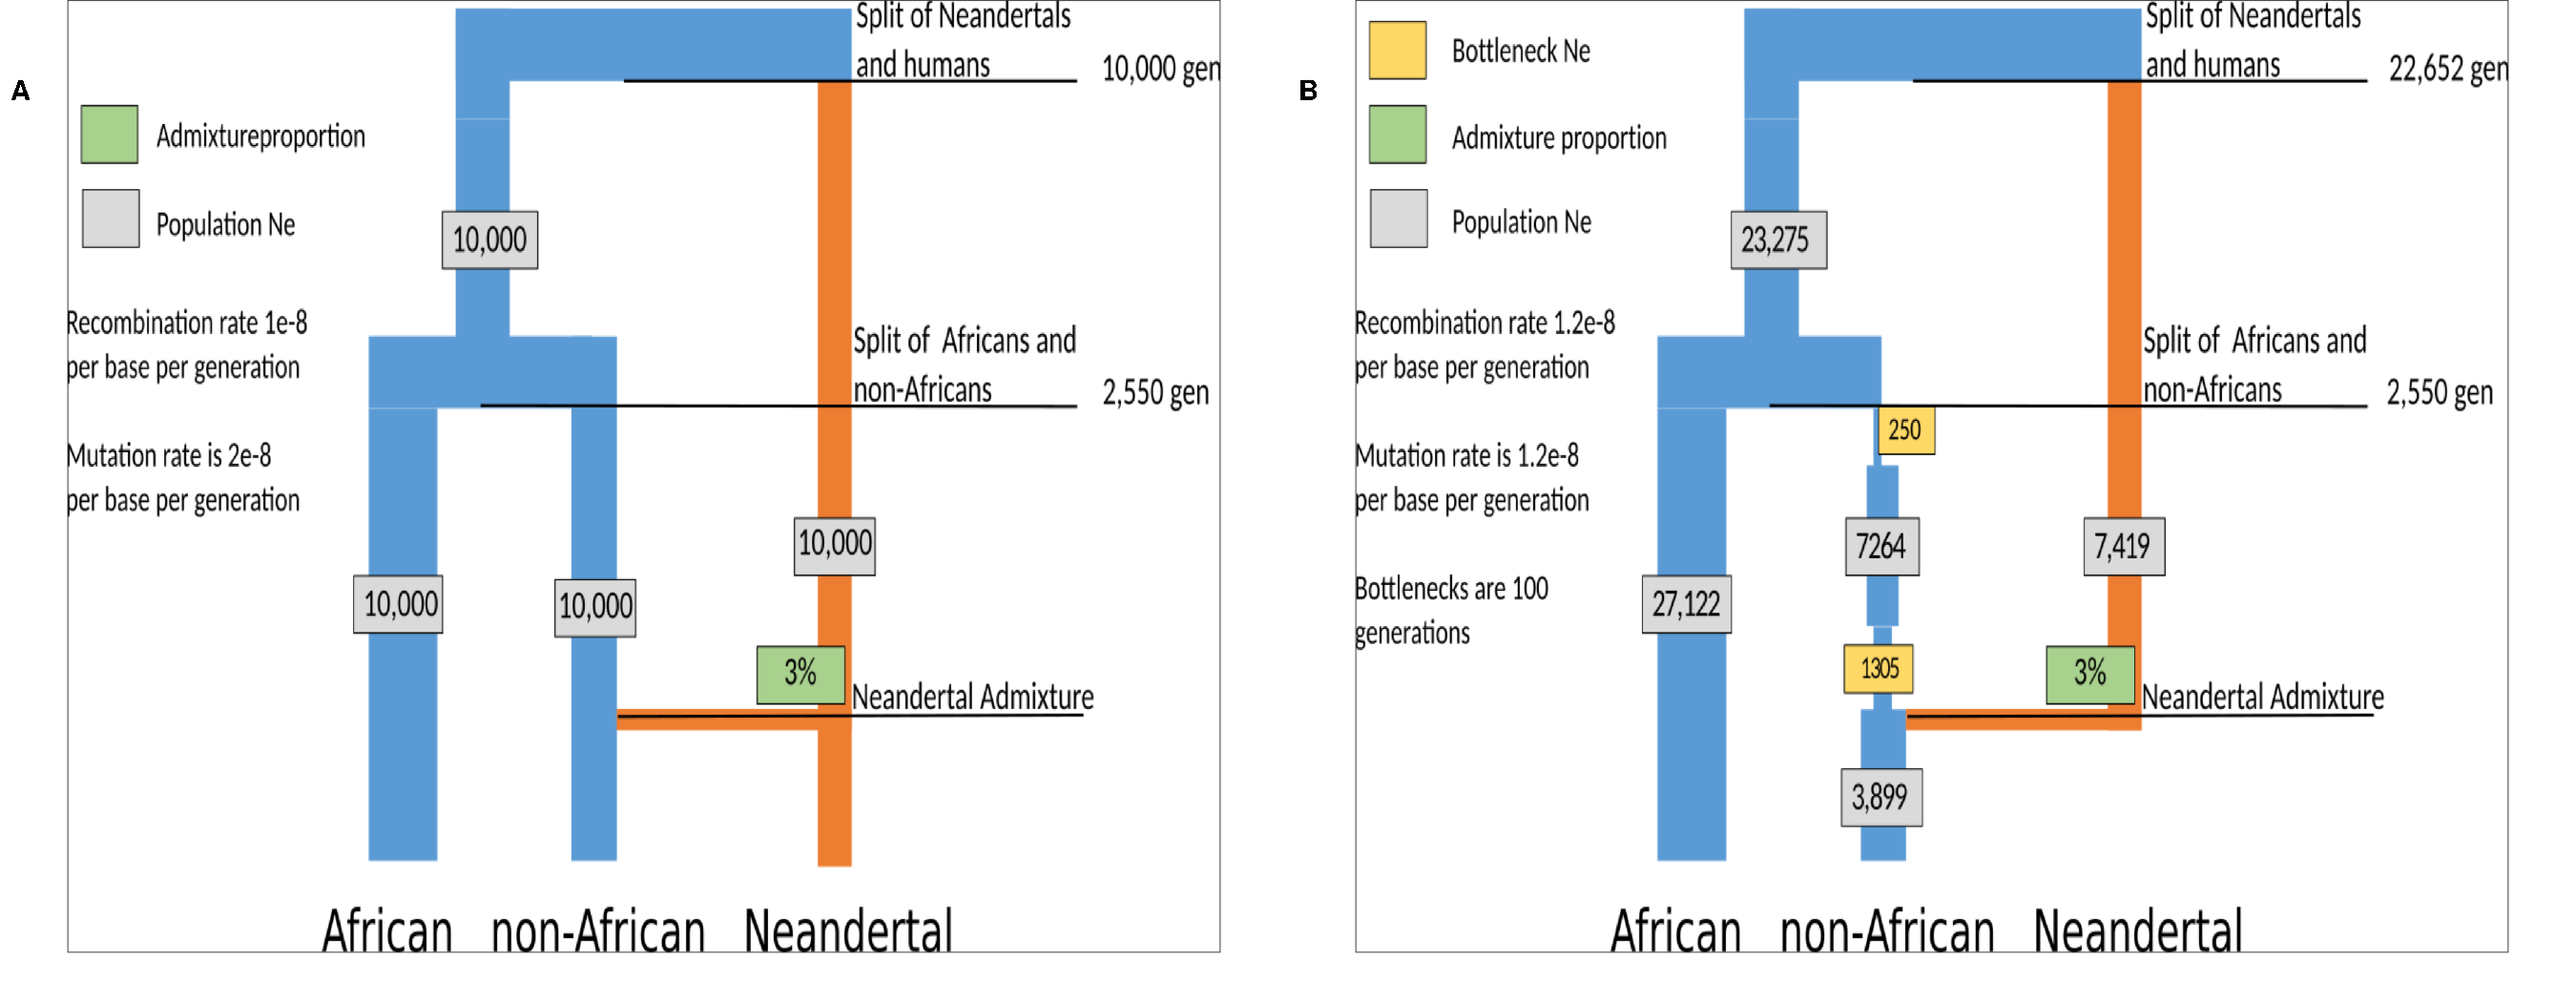
\includegraphics{Admixture_Time_Inference_Paper_Draft_files/figure-latex/Simple_and_Skov.pdf}
\caption{\label{fig:figS1} Demographic models of Neandertal introgression into non-Africans used for the simulations. A) Simple demographic model used for ALD simulations with constant population sizes. B) Complex demographic model with population size changes derived from Skov et al. 2018.}
\end{figure}



\begin{figure}
\centering
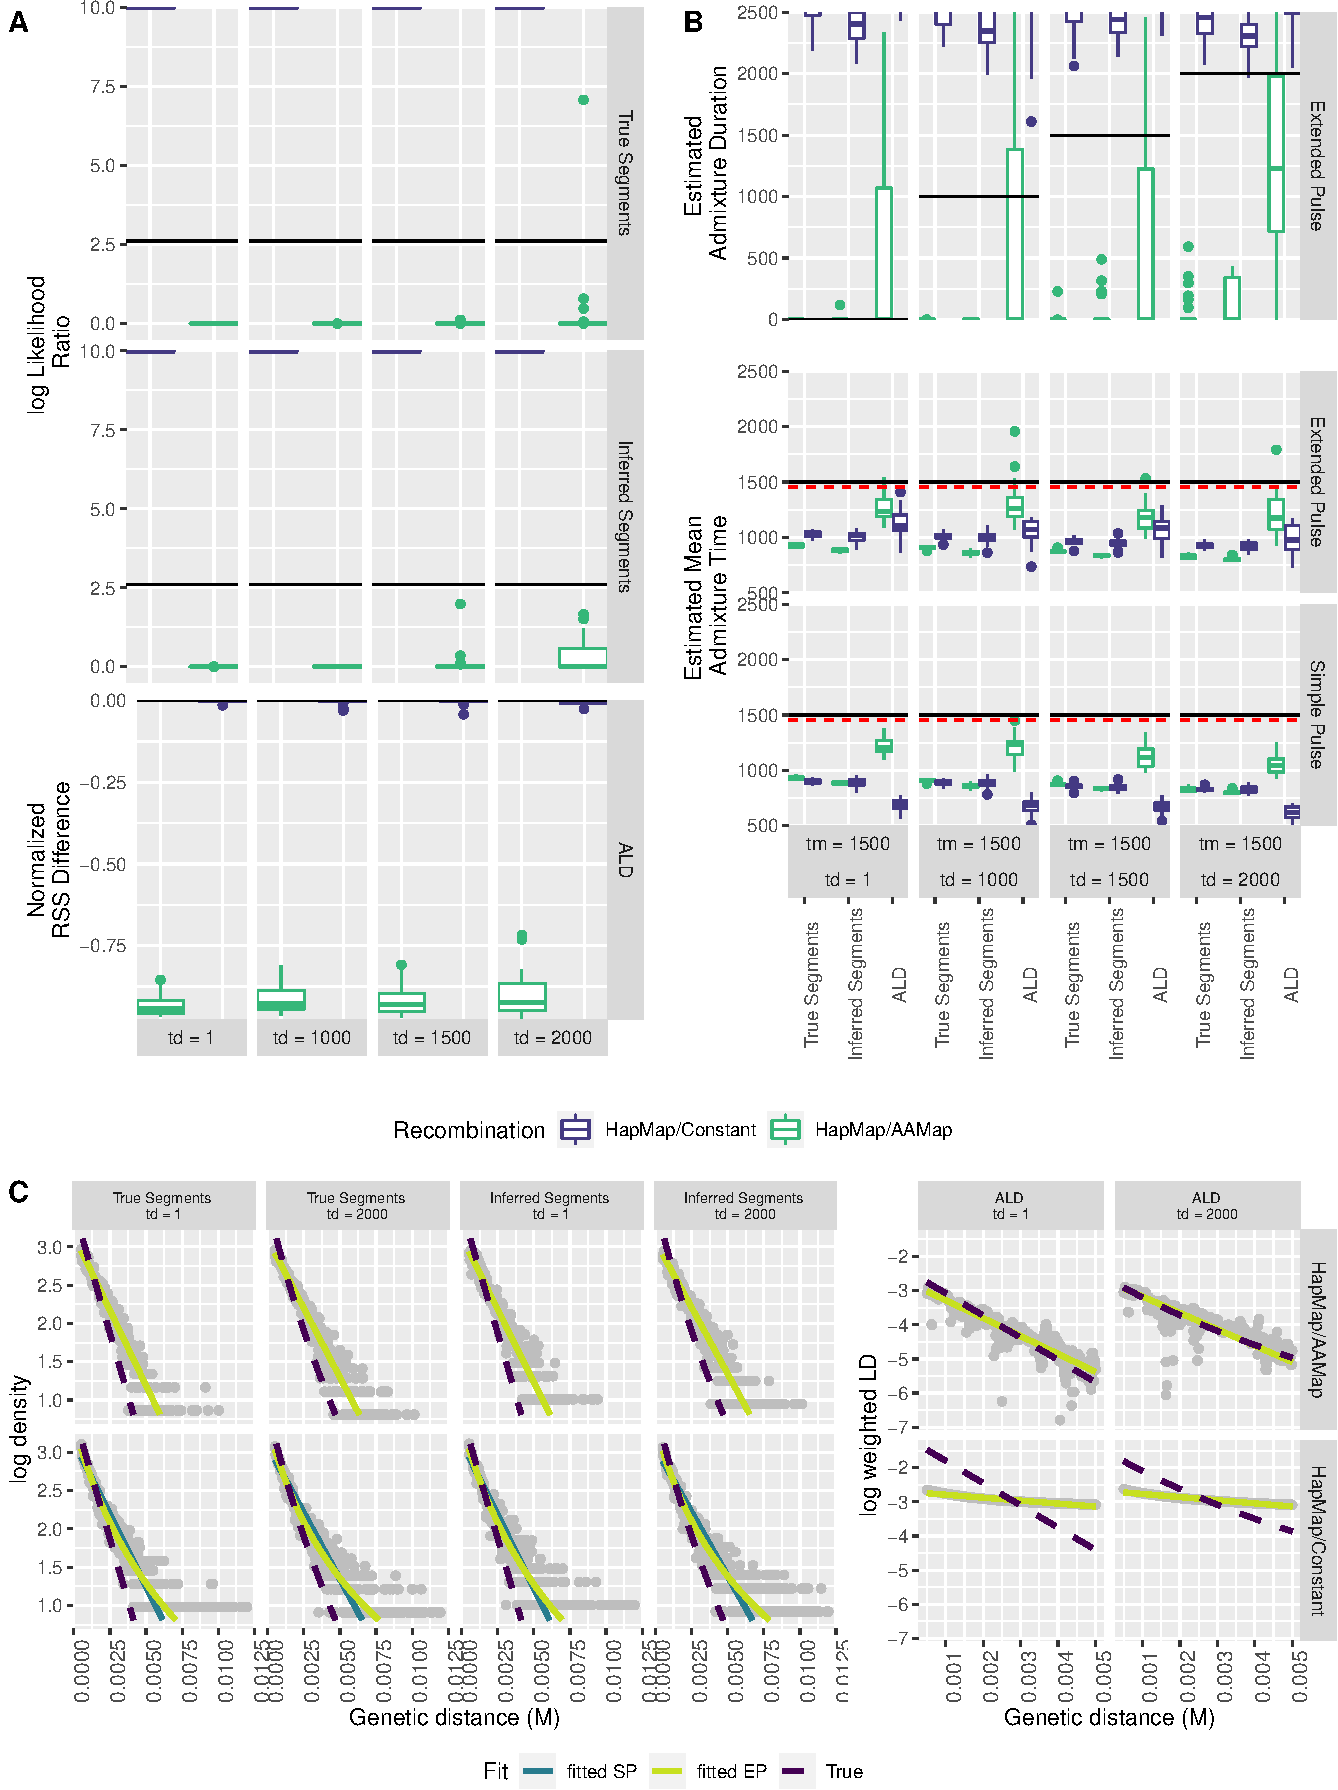
\includegraphics[width=16cm,height=18cm,keepaspectratio]{ATE_Revisions_files/figure-latex/figResult2_all_together_Supplements-1.pdf}
\caption{\label{fig:figResult2_sup} Comparison between the simple and extended pulse one true and inferred segment length and ALD decay estimates using an empirical recombination map (HapMap) for simulations with a fixed mean time ($t_m$) of 1500 generations ago and varying durations ($t_d$). Genetic distances are assigned either using a constant rate or the AAMap . A) log likelihood ratios between the two models for segment data and normalized difference between the residual sum-of-squares between the two models for ALD data. B) Mean time estimates of admixture and extended pulse estimate for admixture duration. Solid black line indicates true $t_m$ and $t_d$, red dotted line indicates migration corrected admixture time ($t_m$(1-m)). C) Comparison of the fit to data between the simple and extended pulse using true and estimated parameters. }
\end{figure}



\begin{figure}
\centering
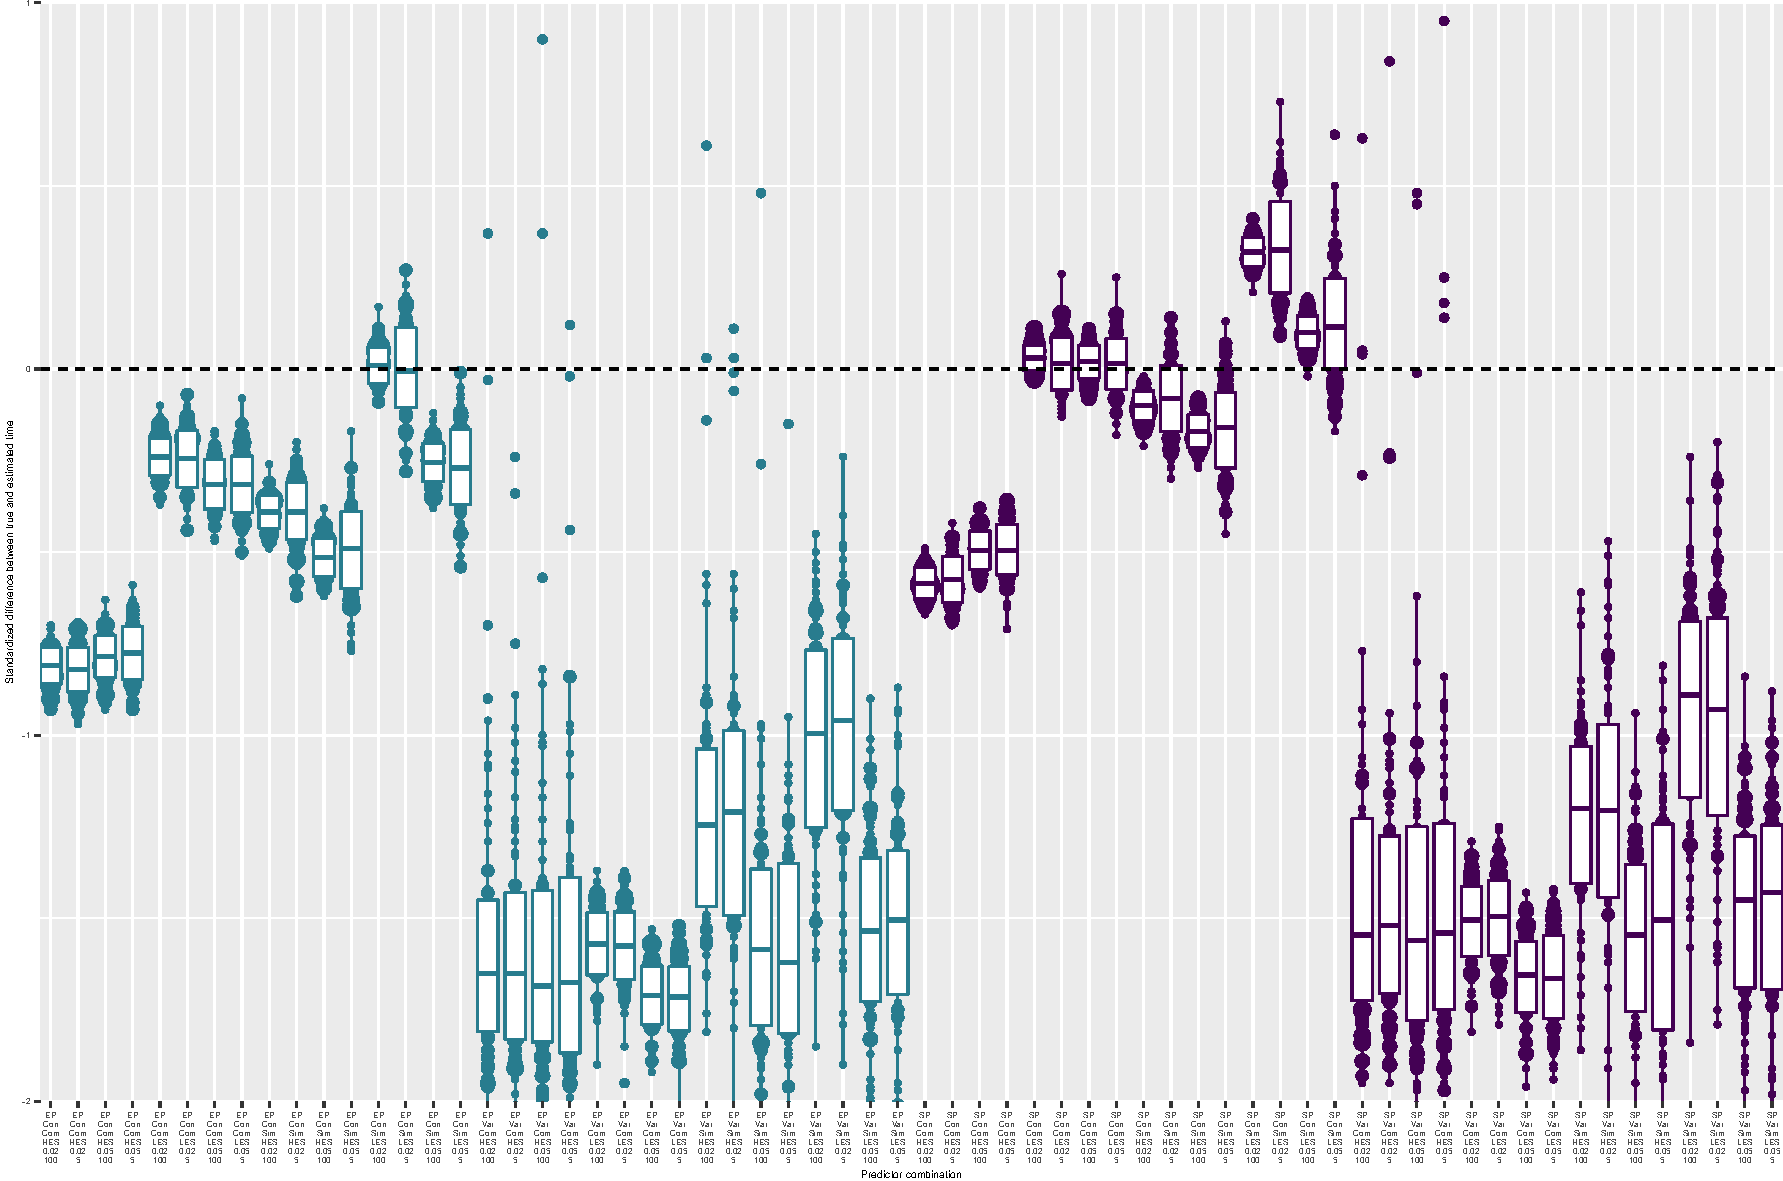
\includegraphics[width=16cm,height=18cm,keepaspectratio]{ATE_Revisions_files/figure-latex/figS2_updated_SP-1.pdf}
\caption{\label{fig:figSGLM_data_SP} Comparison of the standardized difference between true and estimated mean admixture time under the simple pulse model for simulations of all combinations of parameters: ascertainment scheme = LES/HES,   minimal genetic distance ($d_{0}$) = 0.02/0.05 cM, demography = simple/complex (sim/com), recombination = constant/variable (con/var), SNP used 100 \% / 5 \% and the gene flow model = simple pulse/extended pulse (SP/EP). Simulations with a simple pulse gene flow are indicated in purple, extended pulse in turquoise. Each simulation was repeated 100 times. Dotted horizontal line indicates no difference between true and estimated time.}
\end{figure}

\begin{figure}
\centering
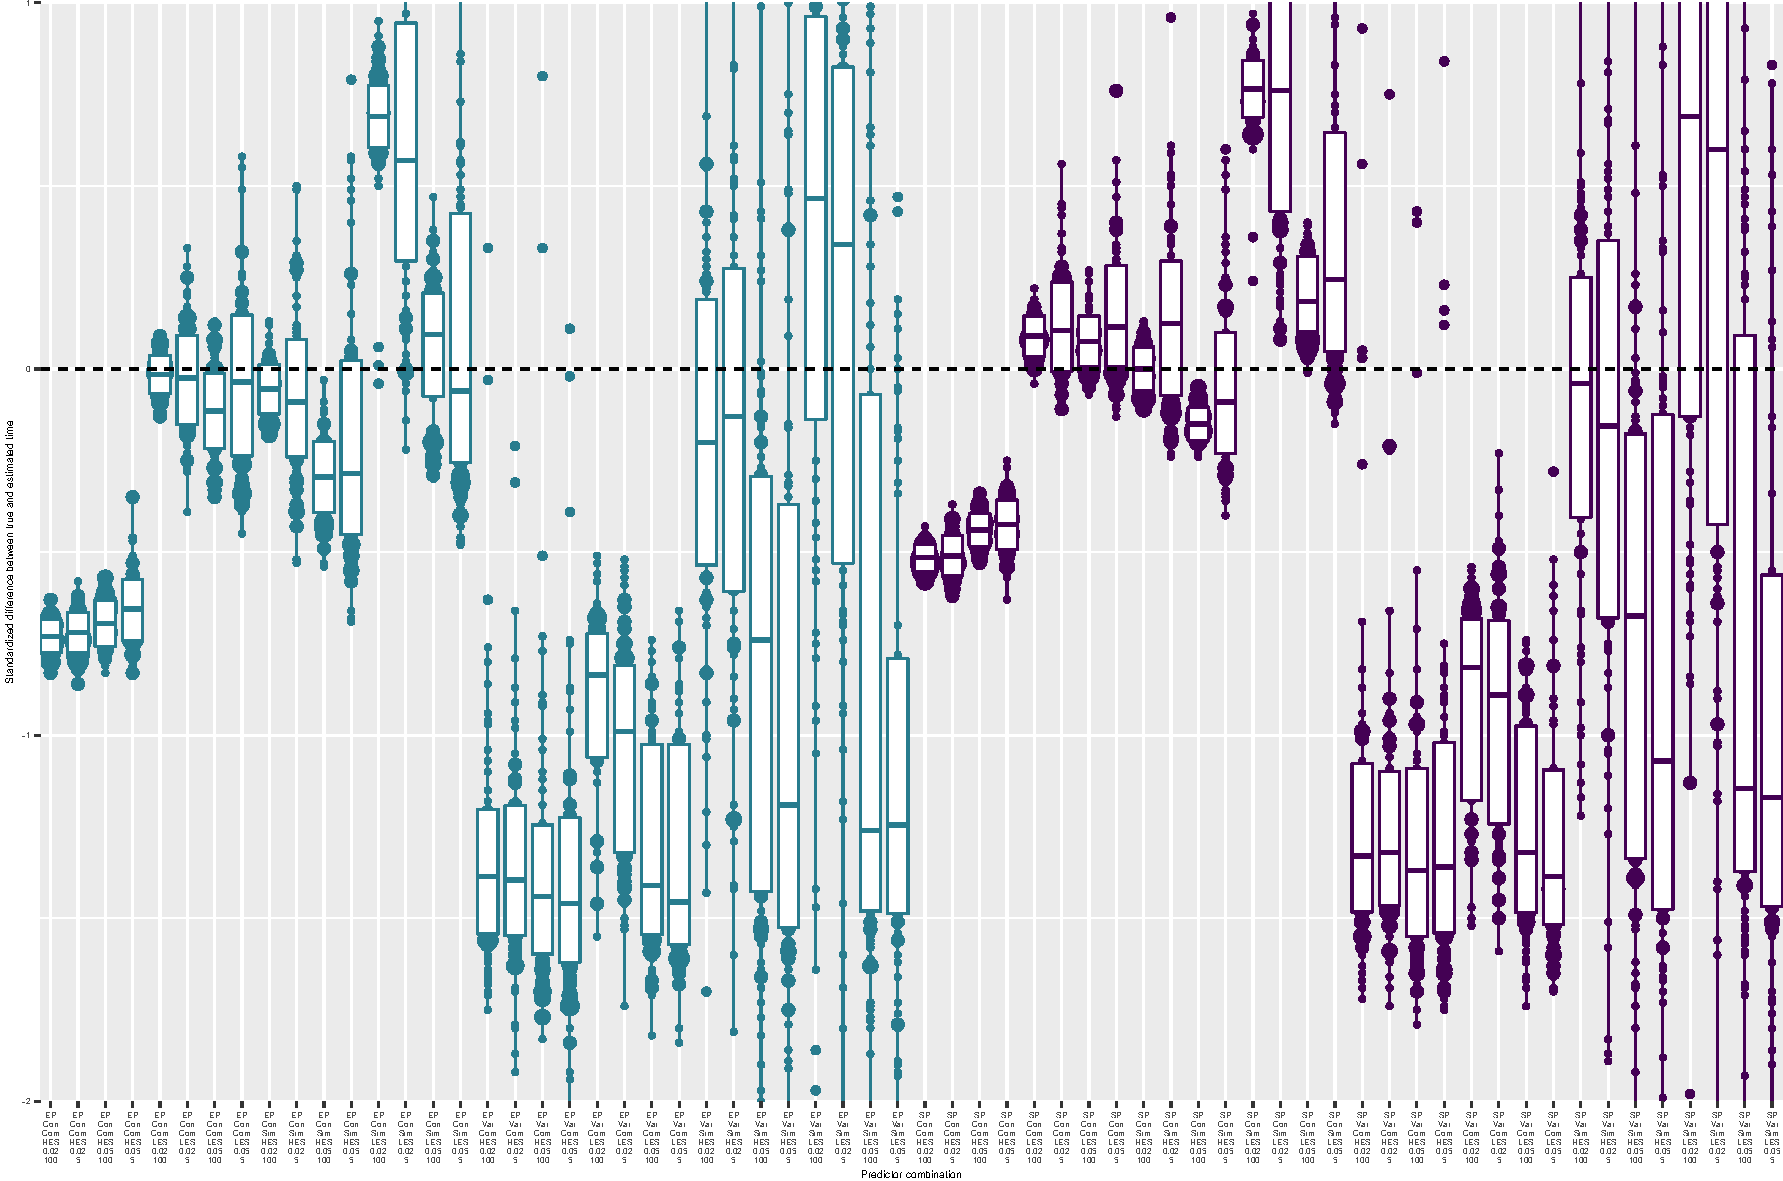
\includegraphics[width=16cm,height=18cm,keepaspectratio]{ATE_Revisions_files/figure-latex/figS2_updated_EP-1.pdf}
\caption{\label{fig:figSGLM_data_EP} Comparison of the standardized difference between true and estimated mean admixture time under the extended pulse model for simulations of all combinations of parameters: ascertainment scheme = LES/HES,   minimal genetic distance ($d_{0}$) = 0.02/0.05 cM, demography = simple/complex (sim/com), recombination = constant/variable (con/var), SNP used 100 \% / 5 \% and the gene flow = simple pulse/extended pulse (SP/EP). Simulations with a simple pulse gene flow are indicated in purple, extended pulse in turquoise. Each simulation was repeated 100 times. Dotted horizontal line indicates no difference between true and estimated time.}
\end{figure}




\begin{figure}
\centering
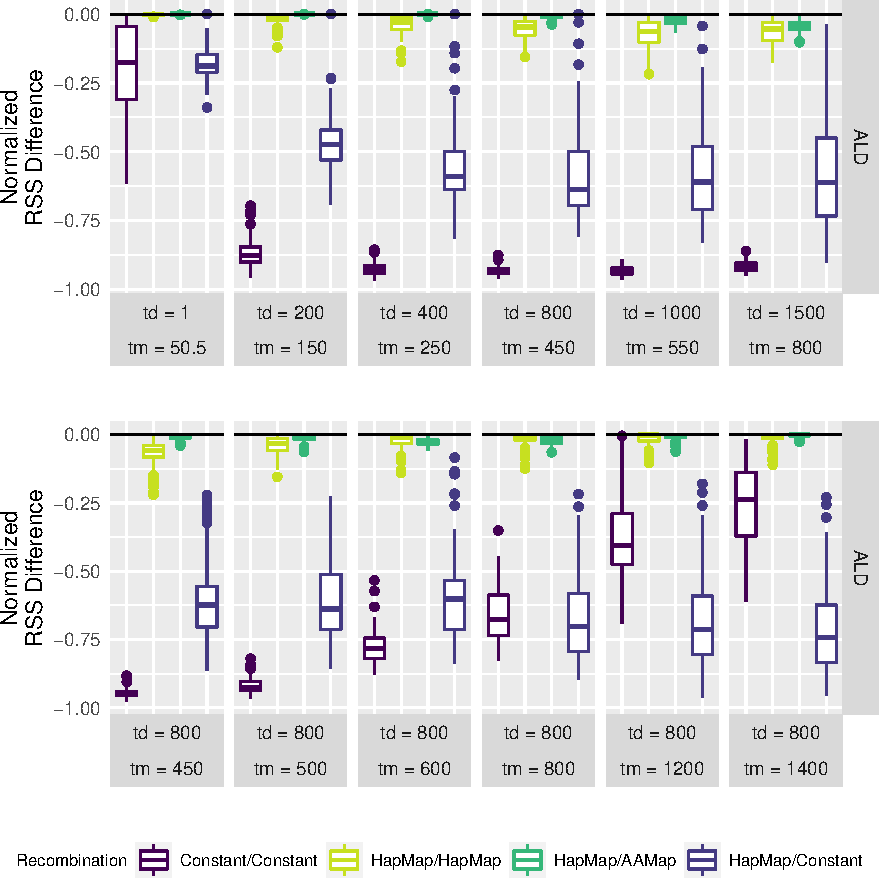
\includegraphics[width=16cm,height=18cm,keepaspectratio]{ATE_Revisions_files/figure-latex/figCloser_Sampling_RSS_Supplement-1.pdf}
\caption{\label{fig:Closer_sampling_supplement} Sampling closer to the admixture event: Normalized difference in the residual-sum-of-squares between the simple pulse fit and extended pulse fit A) Comparison for scenarios sampled 50 generations after the gene flow ended, with different gene flow durations. B) Comparison for scenarios with different sampling times after 800 generations of gene flow.}
\end{figure}

\section{Supplement Tables}


\begin{table}[H]

\caption{\label{tab:table_Supplements_ests_bias}Comparing effect sizes for technical covariates: GLM parameter estimates on the bias between the true and estimated mean admixture time}
\centering

\begin{tabular}[t]{l|l|l|r|r|r}
\hline
model & GLM & covariate & mean & 5.5\% & 94.5\%\\
\hline
 & bias & Standard Model & 0.00 & -0.07 & 0.06\\

 & bias & Extended Pulse & -0.17 & -0.21 & -0.13\\

 & bias & Varying recombination & -1.22 & -1.29 & -1.16\\

 & bias & Complex Demography & -0.27 & -0.33 & -0.22\\

 & bias & d0 = 0.02 & 0.15 & 0.08 & 0.21\\

 & bias & HES & -0.15 & -0.22 & -0.09\\

 & bias & n SNP = 5\% & 0.00 & -0.06 & 0.05\\

 & bias & Interaction n SNP = 5\%/HES & 0.01 & -0.06 & 0.09\\

 & bias & Interaction Complex D./Varying R. & -0.05 & -0.13 & 0.03\\

 & bias & Interaction d0 = 0.02/HES & -0.14 & -0.21 & -0.06\\

\multirow{-11}{*}{\raggedright\arraybackslash Simple Pulse} & bias & Interaction d0 = 0.02/Varying R. & 0.18 & 0.10 & 0.26\\
\cline{1-6}
 & bias & Standard Model & 0.21 & 0.15 & 0.28\\

 & bias & Extended Pulse & -0.11 & -0.15 & -0.07\\

 & bias & Varying recombination & -0.74 & -0.80 & -0.67\\

 & bias & Complex Demography & -0.43 & -0.49 & -0.38\\

 & bias & d0 = 0.02 & 0.38 & 0.31 & 0.45\\

 & bias & HES & -0.18 & -0.25 & -0.11\\

 & bias & n SNP = 5\% & -0.04 & -0.10 & 0.01\\

 & bias & Interaction n SNP = 5\%/HES & 0.05 & -0.03 & 0.13\\

 & bias & Interaction Complex D./Varying R. & -0.44 & -0.52 & -0.36\\

 & bias & Interaction d0 = 0.02/HES & -0.40 & -0.48 & -0.32\\

\multirow{-11}{*}{\raggedright\arraybackslash Extended Pulse tm} & bias & Interaction d0 = 0.02/Varying R. & 0.46 & 0.38 & 0.54\\
\hline
\end{tabular}
\end{table}


\begin{table}[H]

\caption{\label{tab:table_Supplements_ests_deviation}Comparing effect sizes for technical covariates: GLM parameter estimates on absolute deviation between  the true and estimated mean admixture time}
\centering
\begin{tabular}[t]{l|l|l|r|r|r}
\hline
model & GLM & covariate & mean & 5.5\% & 94.5\%\\
\hline
 & abs. deviation & Standard Model & 0.08 & 0.02 & 0.14\\

 & abs. deviation & Extended Pulse & 0.15 & 0.12 & 0.19\\

 & abs. deviation & Varying recombination & 1.26 & 1.19 & 1.32\\

 & abs. deviation & Complex Demography & 0.17 & 0.12 & 0.22\\

 & abs. deviation & d0 = 0.02 & -0.06 & -0.12 & 0.00\\

 & abs. deviation & HES & 0.18 & 0.12 & 0.24\\

 & abs. deviation & n SNP = 5\% & 0.01 & -0.04 & 0.06\\

 & abs. deviation & Interaction n SNP = 5\%/HES & 0.00 & -0.07 & 0.07\\

 & abs. deviation & Interaction Complex D./Varying R. & 0.03 & -0.03 & 0.11\\

 & abs. deviation & Interaction d0 = 0.02/HES & 0.10 & 0.03 & 0.17\\

\multirow{-11}{*}{\raggedright\arraybackslash Simple Pulse} & abs. deviation & Interaction d0 = 0.02/Varying R. & -0.23 & -0.30 & -0.16\\
\cline{1-6}
 & abs. deviation & Standard Model & 0.15 & 0.09 & 0.20\\

 & abs. deviation & Extended Pulse & 0.09 & 0.05 & 0.12\\

 & abs. deviation & Varying recombination & 0.82 & 0.76 & 0.88\\

 & abs. deviation & Complex Demography & 0.02 & -0.03 & 0.07\\

 & abs. deviation & d0 = 0.02 & 0.11 & 0.05 & 0.17\\

 & abs. deviation & HES & 0.10 & 0.04 & 0.16\\

 & abs. deviation & n SNP = 5\% & 0.07 & 0.02 & 0.12\\

 & abs. deviation & Interaction n SNP = 5\%/HES & 0.01 & -0.06 & 0.08\\

 & abs. deviation & Interaction Complex D./Varying R. & 0.28 & 0.21 & 0.35\\

 & abs. deviation & Interaction d0 = 0.02/HES & -0.03 & -0.10 & 0.04\\

\multirow{-11}{*}{\raggedright\arraybackslash Extended Pulse tm} & abs. deviation & Interaction d0 = 0.02/Varying R. & -0.41 & -0.48 & -0.34\\
\hline
\end{tabular}
\end{table}

\begin{table}[H]
\tiny
\caption{\label{tab:table_Supplements_Application_to_Neandertal_data_Estimates} Application to Neandertal data: Estimates}
\centering
\begin{tabular}[t]{l|l|l|l|l}
\hline
  & Model & tm & A & c\\
\hline
Simple Pulse & Simple Pulse & 1682 (1526 - 1839) & 0.019 (0.019 - 0.019) & 0.000182 (0.00016 - 0.000204)\\
\cline{1-5}
Extended Pulse (td=1) & Extended Pulse (td=1) & 1682 (1526 - 1839) & 0.019 (0.019 - 0.019) & 0.000182 (0.00016 - 0.000204)\\
\cline{1-5}
Extended Pulse (td=100) & Extended Pulse (td=100) & 1683 (1527 - 1839) & 0.019 (0.019 - 0.019) & 0.000182 (0.00016 - 0.000204)\\
\cline{1-5}
Extended Pulse (td=200) & Extended Pulse (td=200) & 1685 (1528 - 1841) & 0.019 (0.019 - 0.019) & 0.000182 (0.00016 - 0.000204)\\
\cline{1-5}
Extended Pulse (td=400) & Extended Pulse (td=400) & 1691 (1534 - 1848) & 0.019 (0.019 - 0.019) & 0.00018 (0.000158 - 0.000202)\\
\cline{1-5}
Extended Pulse (td=800) & Extended Pulse (td=800) & 1717 (1558 - 1877) & 0.019 (0.019 - 0.019) & 0.000174 (0.000152 - 0.000196)\\
\cline{1-5}
Extended Pulse (td=1000) & Extended Pulse (td=1000) & 1736 (1575 - 1898) & 0.02 (0.02 - 0.02) & 0.00017 (0.000148 - 0.000192)\\
\cline{1-5}
Extended Pulse (td=1500) & Extended Pulse (td=1500) & 1800 (1633 - 1967) & 0.02 (0.02 - 0.02) & 0.000155 (0.000134 - 0.000177)\\
\cline{1-5}
Extended Pulse (td=2000) & Extended Pulse (td=2000) & 1882 (1707 - 2057) & 0.021 (0.021 - 0.021) & 0.000138 (0.000116 - 0.000159)\\
\cline{1-5}
Extended Pulse (td=2500) & Extended Pulse (td=2500) & 1978 (1794 - 2161) & 0.022 (0.022 - 0.022) & 0.000118 (9.6e-05 - 0.00014)\\
\hline
\end{tabular}
\end{table}

\begin{table}[H]

\caption{\label{tab:table_Supplements_Application_to_Neandertal_data_RSS} Application to Neandertal data: RSS}
\centering
\begin{tabular}[t]{l|r}
\hline
Model & RSS\\
\hline
Simple Pulse & 2.53e-05\\
\cline{1-2}
Extended Pulse (td=1) & 2.53e-05\\
\cline{1-2}
Extended Pulse (td=100) & 2.53e-05\\
\cline{1-2}
Extended Pulse (td=200) & 2.53e-05\\
\cline{1-2}
Extended Pulse (td=400) & 2.53e-05\\
\cline{1-2}
Extended Pulse (td=800) & 2.51e-05\\
\cline{1-2}
Extended Pulse (td=1000) & 2.50e-05\\
\cline{1-2}
Extended Pulse (td=1500) & 2.47e-05\\
\cline{1-2}
Extended Pulse (td=2000) & 2.44e-05\\
\cline{1-2}
Extended Pulse (td=2500) & 2.42e-05\\
\hline
\end{tabular}
\end{table}

\end{document}